\section{Proof of Stake: The Nothing at Stake problem}

At a first glance, Proof of Stake seems to be a great idea. It is more energy efficient than Proof of Work, and it is more democratic in the sense that the more tokens you have, the more say you have in the network.

However, it is not quite comparable to Proof of Work. To understand why, we need to notice the following two properties of PoW:

\begin{itemize}
    \item \textbf{Finite prowess}: In proof of work systems, the prowess (often calculated as the number of puzzles a miner can try) of a miner is limited by the amount of computational power they have. Whether they use COTS, ASICs, FPGAs, all are limited inherently. Whenever a miner sees a fork in the chain, they have a choice to make: which chain to mine on. Should they dedicate their prowess to the \texttt{fork \#1} or should they dedicate their prowess to \texttt{fork \#2}? Or should they mine on both equally? Regardless of their choice of prowess distribution, their total prowess is limited.
    \item \textbf{Wrong choice is costly}: If a miner chooses to mine on the wrong fork, they lose out on the rewards they could have gotten had they mined on the right fork. This is because the right fork will have more blocks, and hence other miners due to longest chain fork-choice rule will focus their effort onto it, making it "the canonical chain" in due time, leaving the wrong fork blocks to be wasted effort / orphaned. 
\end{itemize}

The above two properties in Proof-of-Work chains, coupled with the assumption that each miner will make their own choice of fork-selection independently, make them inherently a good canonicalization machine, i.e. given enough time all forks will converge to a single chain. 

However, in Proof of Stake, the above two properties are not true. The prowess of a validator is not limited by computational power, but by the amount of tokens they have staked. Any validator can freely attest on both the forks. Secondly, since they are not making a choice here, there is no concept of "wrong choice" being costly. This leads to a problem called "Nothing at Stake".

\subsection{No penalties = No canonicalization}

In many early (all chain-based) proof of stake algorithms, including \href{https://www.peercoin.net/}{Peercoin}, there are only rewards for producing blocks, and \textbf{no penalties}. This has the unfortunate consequence that, in the case that there are multiple competing forks, it is in a validator's incentive to try to make blocks on top of every fork at once, just to be sure.

The result is that if all actors are narrowly economically rational, then even if there are no attackers, a blockchain may never reach consensus on a "canonical state", and all validators will keep building on both forks. \hl{If there is an attacker, then the attacker need to only overpower the altruistic nodes (who would exclusively stake on the original chain), and not rational nodes (who would stake on both the original chain and the attacker's chain), in contrast to proof of work, where the attacker must overpower both altruists and rational nodes.}

\subsection{Example: The 1\% attacker}
\todo{Show how a person controlling >0\% stake can canonicalize the wrong fork and thus you cannot trust any fork until its made canonical}

\subsection{The Tragedy of the Commons}
The Tragedy of the Commons is a concept which states that if many people enjoy unfettered access to a finite, valuable resource, such as a pasture, they will tend to overuse it and may end up destroying its value altogether. Even if some users exercised voluntary restraint, the other users would merely replace them, the predictable result being a "tragedy" for all.

\begin{wrapfigure}{r}{0.70\textwidth}
    \centering
    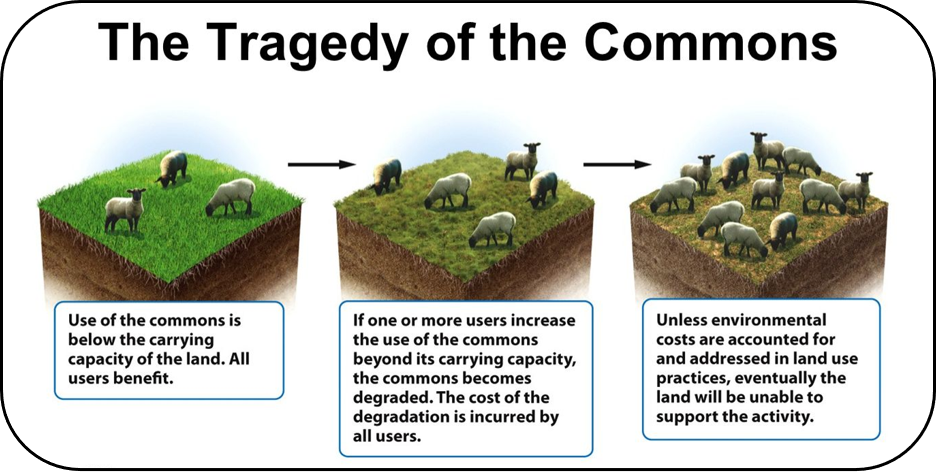
\includegraphics[width=0.70\textwidth]{general-problems/assets/tragedy-of-the-commons.png}
    \caption{Tragedy of the commons}
    \label{fig:tragedy-of-the-commons}
\end{wrapfigure}

In the context of Proof of Stake, each individual stakeholder might only have a 1\% chance of being "pivotal" (i.e. being in a situation where if they participate in an attack then it succeeds and if they do not participate it fails), and so the bribe needed to convince them personally to join an attack would be only 1\% of the size of their deposit; hence, the required combined bribe would be only 0.5-1\% of the total sum of all deposits. Additionally, this argument implies that any zero-chance-of-failure situation is not a stable equilibrium, as if the chance of failure is zero then everyone has a 0\% chance of being pivotal.

\subsection{Simulating the "wrong choice is costly"}
There are two ways in which one can try solving the "Nothing at Stake" problem, both of which involve making the "wrong choice" costly:

\begin{itemize}
    \item \textbf{Slasher}: In the Slasher algorithm, if a validator is caught signing two conflicting blocks on two different forks, they lose their part / entire stake. \todo{requires elaboration, see why they call it too harsh}
    \item \textbf{Casper FFG}: Every validator is forced to choose a fork to validate on. If there are two competing chains, A and B, then if a validator creates a block on B, they get a reward of +R on B, but the block header can be included into A (in Casper this is called a "dunkle" or \emph{proof of malfeasance}) and on A the validator suffers a penalty of -F (possibly F = R). \todo{show in Casper design how this is done}
\end{itemize}
% \colorbox{Highlight}{If there is an attacker, then the attacker need only overpower altruistic nodes}